\chapter{Feasibility Study of a Pixelated LArTPC for the \dune Near Detector}
\label{chap:dune-nd}

With \AC\ selected as  the \lar\ component of the \dune\ near detector (ND), there were two main question that needed to be addressed:
\begin{enumerate}
	\item Is a pixelated \lartpc\ feasible?
	\item Can the \lar\ detector handle the high rates?
\end{enumerate}
Number one is addressed in Chapter~\ref{chap:viper}.
This chapter will address question number two.


\section{The High-Multiplicity Environment of the \dune\ Near Detector}
\label{sec:dune-nd_multiplicity}

One of the main goals of \dune\ is to measure the Dirac CP violation phase $\delta_{\m{CP}}$ provided it has a non-degenerate value.
To reach a $3 \sigma$ sensitivity for a \SI{75}{\percent} coverage of the $\delta_{\m{CP}}$ parameter space, an exposure of \SI{1320}{\kilo\tonne\mega\watt years} is required (see Figure~\ref{fig:dune-nd_cpv-sens}).~\cite{dune2}
Assuming the reference design of a \SI{40}{\kilo\tonne} far detector and a \SI{1}{\mega\watt} beam results in a data taking time of \SI{33}{years}.
Therefore, to make the data taking time shorter, a beam $> \SI{1}{\mega\watt}$ is required.
On the other hand, combining the numbers of the reference design in~\cite{dune2}, the event rate in the ND amounts to \SI{0.1}{evt\per\tonne\per\mega\watt} leading to significant event pile-up.
This number does not include rock events---secondary particles produced by beam neutrino interactions in the surrounding material, entering the detector.
The neutrino beam flux is depicted in Figure~\ref{fig:dune-nd_flux}.

\begin{figure}[htb]
	\centering
	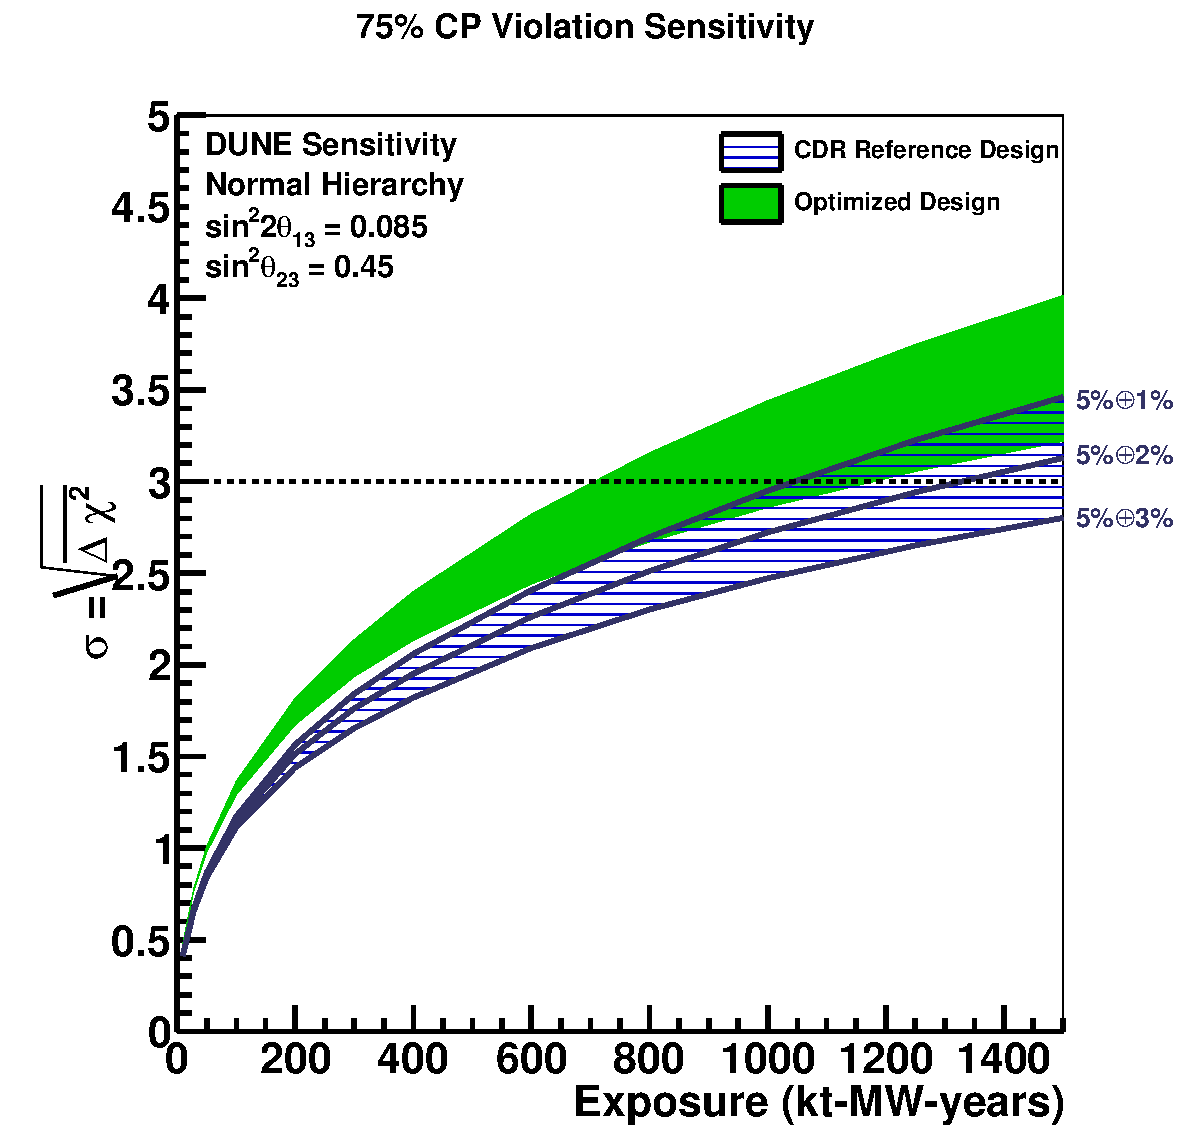
\includegraphics[width=.5\textwidth]{dune-nd/dune_cpv75_exp_syst}
	\caption{Expected sensitivity of \dune\ to discovery of CP violation, i.e.\ $\delta_{\m{CP}} \neq\ 0\ \m{or} \pi$ as a function of exposure in \si{\kilo\tonne\mega\watt years}, assuming equal running in neutrino and antineutrino mode.~\cite{dune2}}
	\label{fig:dune-nd_cpv-sens}
\end{figure}

\begin{figure}[htb]
	\centering
	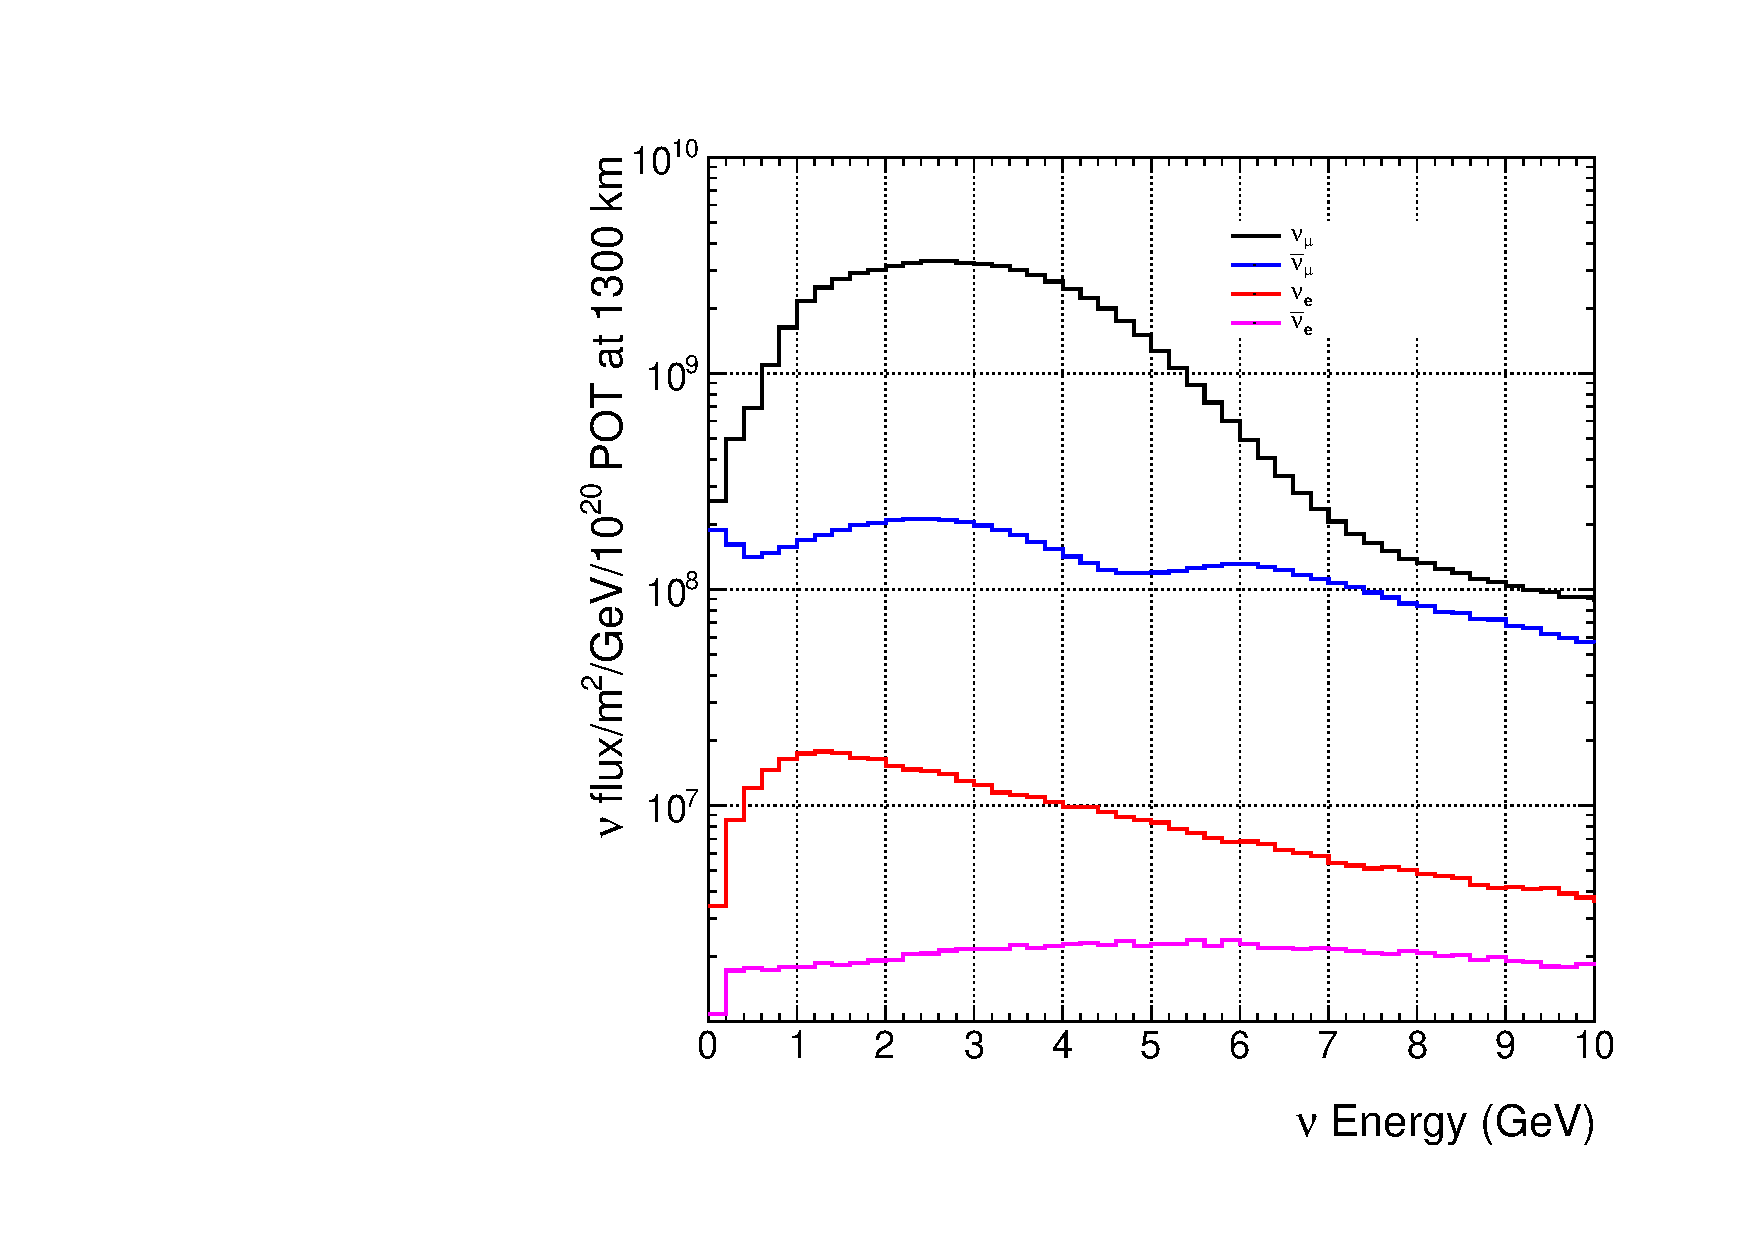
\includegraphics[width=.49\textwidth]{pile-up/FHC_230kA}
	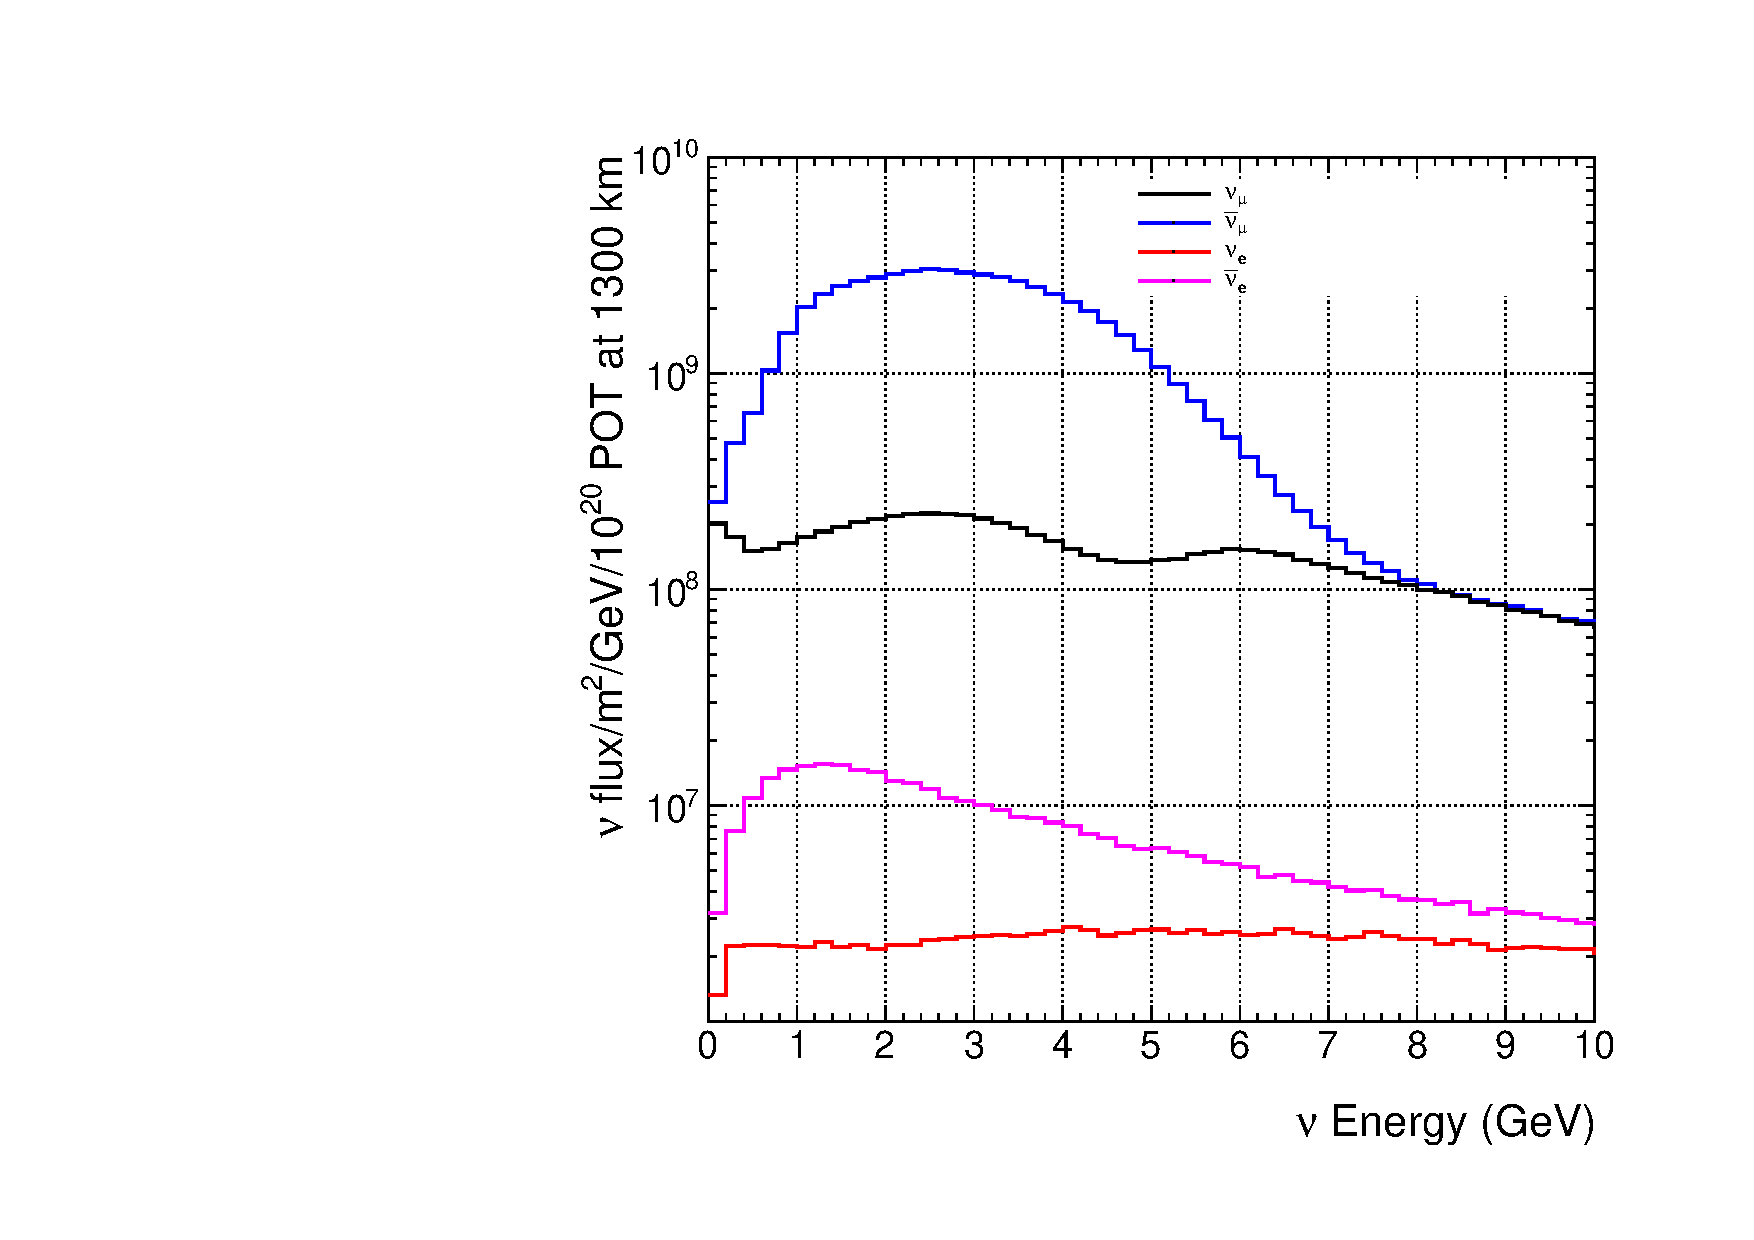
\includegraphics[width=.49\textwidth]{pile-up/RHC_230kA}
	\caption{Neutrino fluxes for the reference beam design operating in neutrino mode (left) and antineutrino mode (right), generated with a \SI{120}{\giga\electronvolt} primary proton beam.~\cite{dune2}}
	\label{fig:dune-nd_flux}
\end{figure}


\section{The Argon Box Simulation Tool}
\label{sec:dune-nd_argon-box}

Argon Box\footnote{\url{https://github.com/dadwyer/argon_box}} was developed with the goal of providing an easy-to-use simulation of particle interactions in \lar\ component of the ND.
At the time of this writing its feature set is quite limited, in particular it does not incorporate any other detector materials except for the box of argon.
Primary particles can either be provided by a particle gun (e.g.\ $e^-$, $n$, $p$, $\mu^+$) or in form of a \emph{HEPEVT} file---a file format standard for passage of particle events between different simulation tools.
For this study, several million neutrino events were produced with the GENIE\footnote{\url{https://genie.hepforge.org}} neutrino event generator.
Secondary particle transport and interaction in Argon Box is performed by Geant4.\footnote{\url{http://geant4.cern.ch}}
Finally, the energy deposition in \lar\ is voxelised and stored together with all the necessary ancillary information about the depositing particle.
The data is stored in the tree format of the ROOT data analysis framework.\footnote{\url{https://root.cern}}
This allows for convenient further processing using ROOT.


\section{$\pi^0$ pile-up study}
\label{sec:dune-nd_pile-up}

A significant amount of $\pi^0$ are produced in several resonant and coherent neutrino interactions (see Section~\ref{sec:nu-detection_interactions} and~\cite{dune2}).
They decay according to
\begin{IEEEeqnarray}{rCl}
	\pi^0 & \qraq & \gamma + \gamma
\end{IEEEeqnarray}
with a branching ratio of \SI{98.8}{\percent}\cite{pdg}.
The photons subsequently produce electromagnetic showers in \lar\ (see Section~\ref{sec:nu-detection_fs}).
At the energies of the \dune\ beam (see Figure~\ref{fig:dune-nd_flux}), most showers do not deposit a homogenous cone of charge but rather a lot of individually resolvable $e^{\pm}$ tracks.
More importantly, there often are significatn gaps in betweend these charge clusters.
A main challenge of shower reconstruction is to associate these well separated charge blobs to the correct event.
Misidentiions lead to a misreconstruction of the neutrino energy.
The resulting discrepancy to the true neutrino energy has the potential to skew the measured energy spectrum and, thus, influence the oscillation measurements.
The complexity of reconstruction paired with the potential impact on the physics measurements makes photons produced by $\pi^0$ decays a good sample to study the robustness to pile-up of a pixelated \lartpc\ in the \dune\ ND environment.

To investigate the effects of pile-up on energy reconstruction, a working reconstruction algorithm is necessary.
However, at the time of writing, official reconstruction tools were only available for \lartpc s read out by wire planes.\footnote{\url{http://larsoft.org}}
Therefore, a rather primitive algorithm for true 3D space points was implemented, under the assumption that a positive outcome of such a pile-up study would imply an even better performance of a more sophisticated reconstruction.
This algorithm is explained in the following.
All its parameters are listed in Table~\ref{tab:dune-nd_pile-up-params}.

The basic underlying assumption is that a non-multiplexed pixel readout will yield unambiguous 3D space points of charge deposition with a given resolution, depending on the geometry of the pixel plane, time resolution of the readout electronics, and charge transport effects.
Furthermore, it is assumed that EM shower can be identified and their starting point and direction reconstructed with negligible errors and inefficiencies, i.e.\ this information is taken from the simulation truth.
A cone is calculated in the direction of the shower with its tip at the first charge deposition of the initial photon.
The opening angle and longituginal extent of the cone were optimised by looking at the distributions of the distance from the starting point and angle w.r.t. the direction of the shower.
The finite resolution of the detector is emulated by voxelising the charge deposition with the corresponding resolution in all three spatial coordinates.
This leads to problems near the tip of the cone where the transversal extent is lower than the voxel dimensions.
In particular, it can happen that most of the initial charge is shifted outside the cone.
Furthermore, multiple scattering at lower energies makes the cone model suboptimal near the tip.
Therefore, the acceptance volume for the reconstruction is taken as the union of the cone with a cylinder around the direction of the shower of the same longitudinal extent as the cone.

\begin{table}[htb]
	\centering
	\caption{Parameters of the $\pi^0$ pile-up simulation.}
	\label{tab:dune-nd_pile-up-params}
	\begin{tabu} to \textwidth {|l|S|}
		\hline
		{Beam direction} &			{$Z$ (positive)} \\
		\hline
		{Gravitation} &				{$Y$ (negative)} \\
		\hline
		{Resolution $X$} &			\SI{3}{\milli\metre} \\
		\hline
		{Resolution $Y$} &			\SI{3}{\milli\metre} \\
		\hline
		{Resolution $Z$} &			\SI{3}{\milli\metre} \\
		\hline
		{Target volume $X$} &		\SIrange{-1000}{5000}{\milli\metre} \\
		\hline
		{Active volume $X$} &		\SIrange{0}{4000}{\milli\metre} \\
		\hline
		{Fiducial volume $X$} &		\SIrange{300}{3700}{\milli\metre} \\
		\hline
		{Target volume $Y$} &		\SIrange{-1000}{3500}{\milli\metre} \\
		\hline
		{Active volume $Y$} &		\SIrange{0}{2500}{\milli\metre} \\
		\hline
		{Fiducial volume $Y$} &		\SIrange{300}{2200}{\milli\metre} \\
		\hline
		{Target volume $Z$} &		\SIrange{-4000}{5000}{\milli\metre} \\
		\hline
		{Active volume $Z$} &		\SIrange{0}{5000}{\milli\metre} \\
		\hline
		{Fiducial volume $Z$} &		\SIrange{300}{4700}{\milli\metre} \\
		\hline
		{Detection threshold} &		\SI{0.1}{\mega\electronvolt} \\
		\hline
		{Cone extent} &				{$10 X_{\m{0}} = \SI{1400}{\milli\metre}$} \\
		\hline
		{Cone half opening angle} &	\SI{15}{\degree} \\
		\hline
		{Cylinder radius} &			\SI{25}{\milli\metre} \\
		\hline
		{Beam intensity} &			{$\SI{2}{\mega\watt} \widehat{=} \SI{0.2}{evt\per\tonne}$} \\
		\hline
	\end{tabu}
\end{table}

Argon Box propagates the neutrino interaction events it gets from GENIE through liquid argon, the output is a ROOT tree of neutrino interaction events.
To get a realisitc simulation of beam events in the detector, these events need to be distributed randomly in time and space.
Beam spills are simulated by drawing the number of events for each spill from a Poisson distrubition whose mean is calculated from the beam intensity and the target mass.
The resulting number of events is taken from the Argon Box ROOT tree and their vertices are placed within the \lar\ volume at coordinates drawn from a uniform distribution.

Three different argon volumes are assumed for the simulation: target, active, and fiducial volume.
The actual detector dimensions are represented by the active volume.
It is inside the target volume which is the volume within which the neutrino vertices are placed randomly.
This is done as a crude emulation of rock events, secondary particles from beam neutrino interactions outside the detector volume.
The additional target mass is \SI{1}{\metre} in all four directions transverse to the beam, and \SI{4}{\metre} in upstream beam direction.
Finally, a fiducial volume \SI{0.3}{\metre} ($\approx 2 X_{\m{0}}$) smaller than the active volume on all six faces is defined.
Without the latter, there is a significant number of photons produced by $pi^0$ decays inside the detector but only showering outside the detector.
Table~\ref{tab:dune-nd_pile-up-params} contains a summary of all the \lar\ volume dimensions.

\begin{figure}[htb]
	\centering
	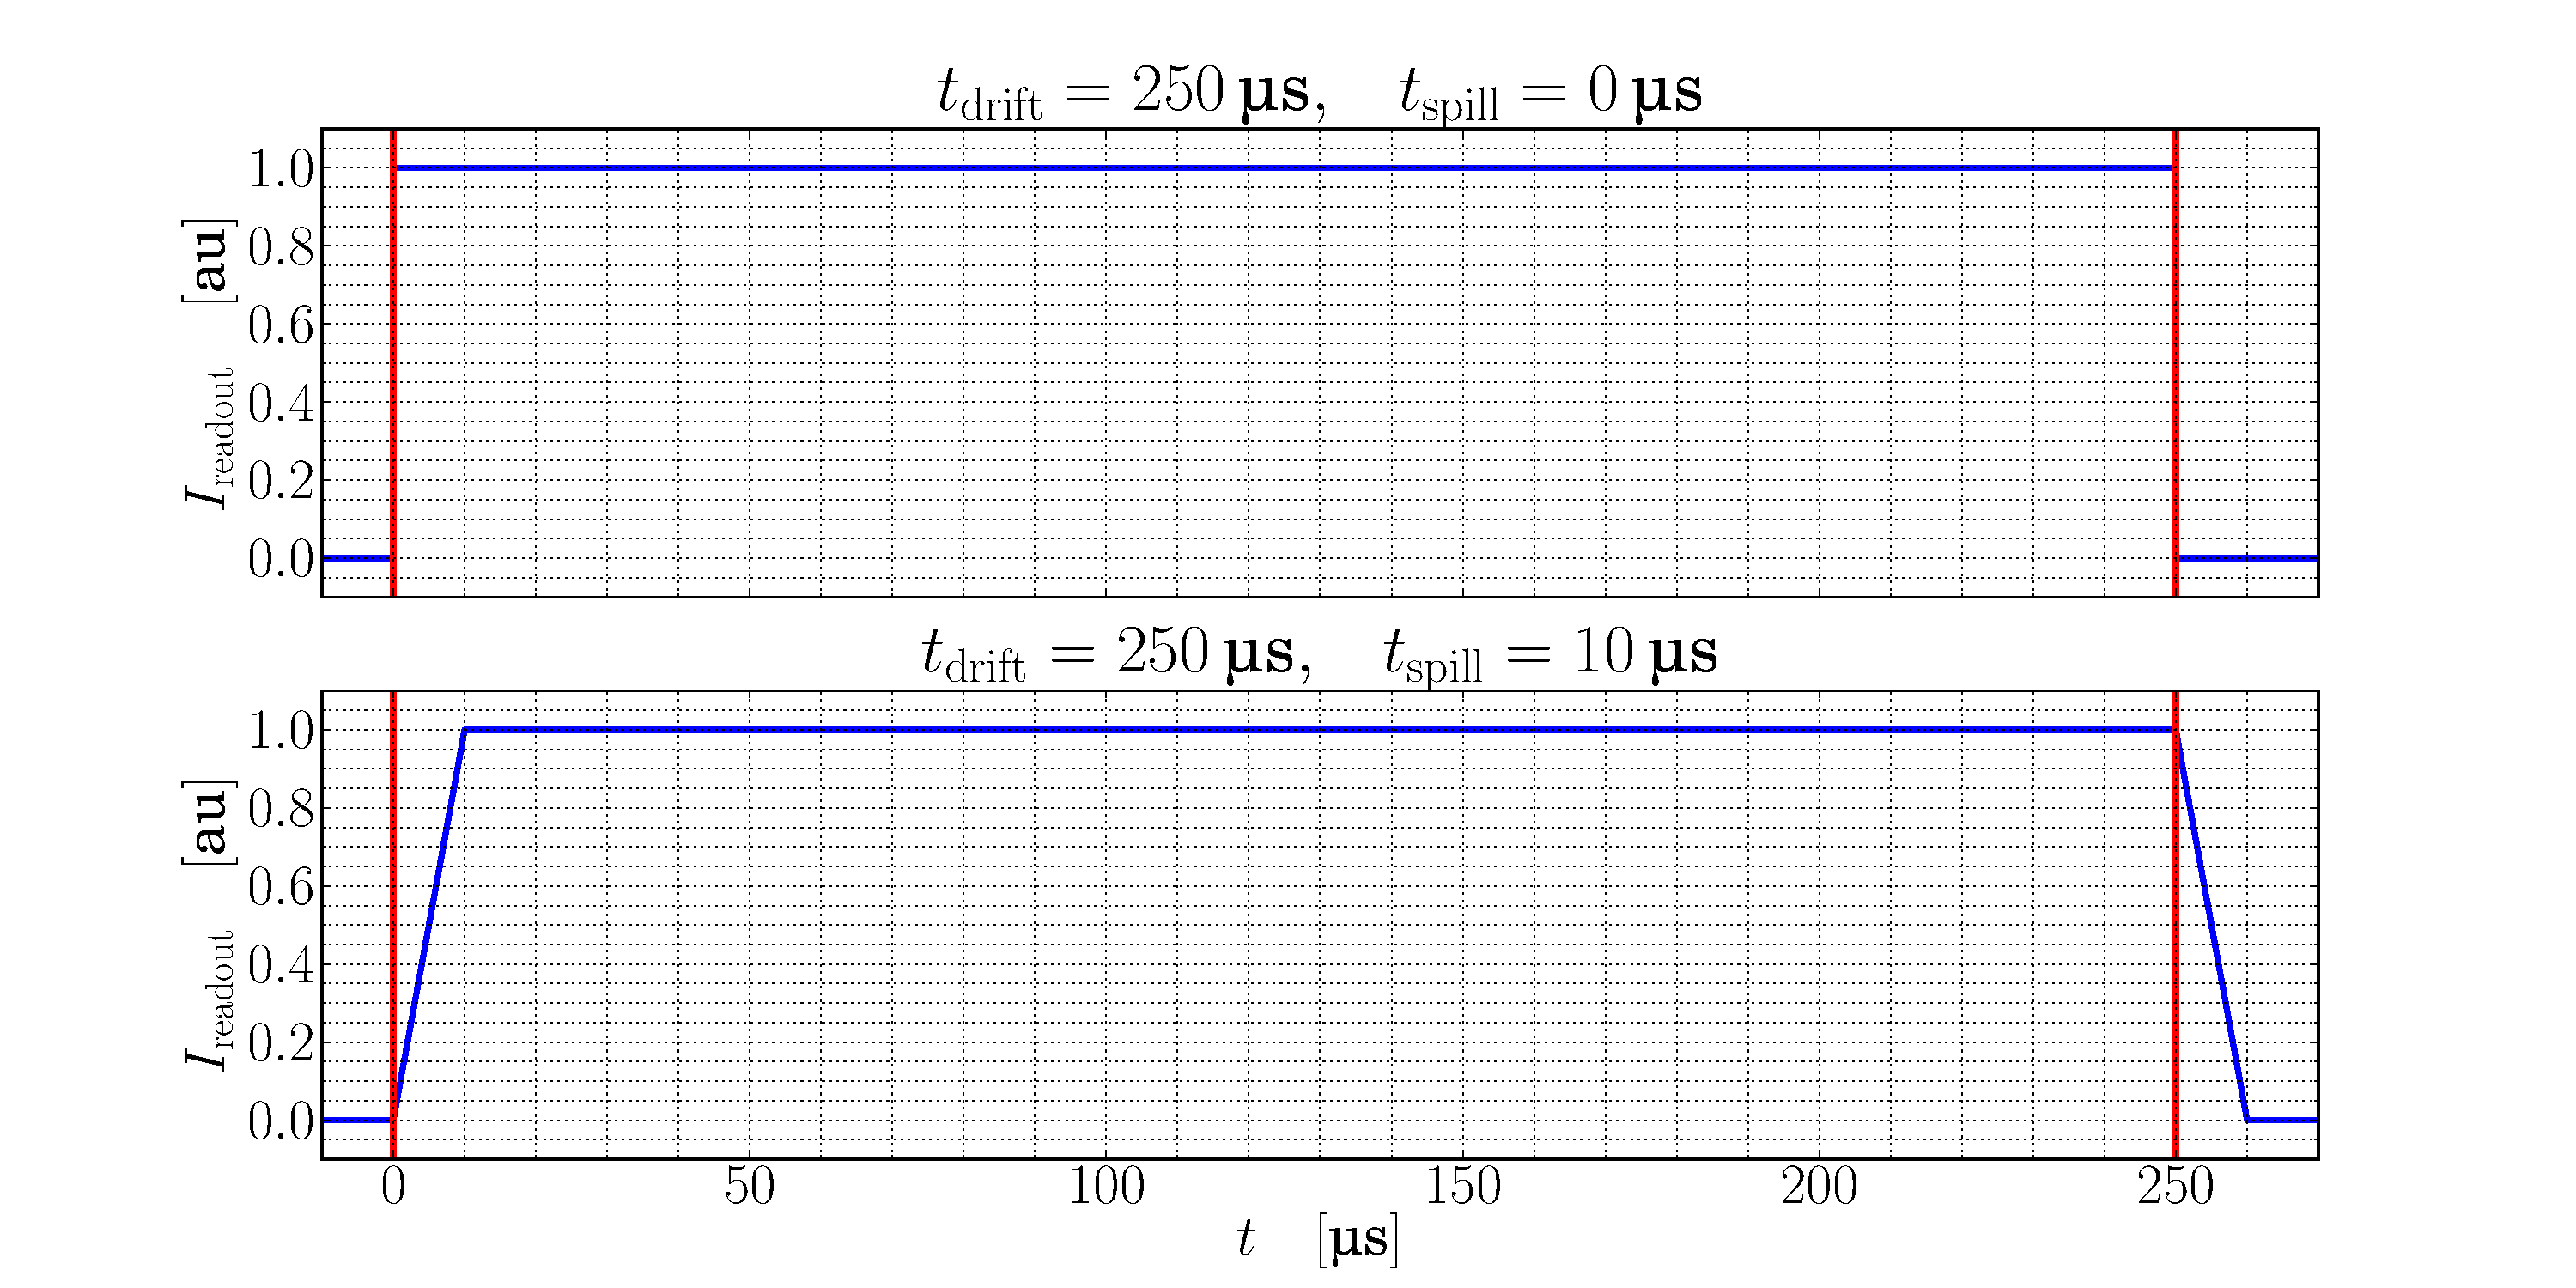
\includegraphics[width=\textwidth]{pile-up/charge_flux}
	\caption{Average current collected by the readout for one spill as a function of time.
	The current is given in arbitrary but equal units for both plots.
	The upper plot assumes the whole charge is deposited instantaneously while for the lower plot, the actual spill duration from~\cite{dune2} is used.}
	\label{dune-nd_charge-flux}
\end{figure}

After all events of one spill are placed inside the target volume, all $pi^0$ photons produced inside the fiducial volume are reconstructed using the cone algorithm.
All energy depositions inside the active volume are considered.
To assess the performance of the performance of the algorithm, the following quantities are computed for each photon:
\begin{itemize}
	\item[Efficiency] Ratio of correctly accepted energy deposition inside the cone-cylinder union to total true energy deposition of the photon.
		This is a measure for the performance of the reconstruction and can be used to ensure optimum tuning of the union parameters.
	\item[Purity] Ratio of correctly accepted energy deposition inside the cone-cylinder union to total accepted energy deposition inside the union.
		This is a measure for event pile-up.
		The higher the amount of charge deposition from other events inside the union, the lower the purity.
\end{itemize}
Using this general definition of purity leads to quite mediocre results.
However, there are some assumptions that can be taken even without knowing the actual reconstruction algorithm.
The incorrectly accepted energy deposition inside the cone-cylinder union can be limited to energy deposited by other events; misidentified energy from the same event does not affect the total reconstructed neutrino energy.
From results of earlier experiments~\cite{sauce}, the muon reconstruction can be assumed to be very efficient.
Assuming \SI{100}{\percent} reconstruction efficiency for muons and \SI{0}{\percent} for all other particles can therefore serve as a lower limit for the purity.
It can be calculated by ignoring misidentified muon energy depositions.
On the other hand, an upper limit for the purity can be calculated by assuming \SI{100}{\percent} reconstruction efficiency for all charged particles and \SI{0}{\percent} for neutral particles ($\pi^0$ and $\gamma$).
This is calculated by only taking into account misidentified energy deposited by neutral particles.
Assuming \SI{0}{\percent} reconstruction efficieny for neutral particles might lead to a slight underestimation of purity.
However, this effect should be more than compensated by the overestimation of the charged particle reconstruction efficiency, given the highly complex nature of reconstructing unconnected clusters from neutral particles.
Therefore, this upper purity limit should hold at least in the near future.

\begin{figure}[htb]
	\centering
	\includegraphics[width=\textwidth]{pile-up/2MW/eff_pur}
	\caption{Efficiency (accepted true over total true energy deposition) and purity (accepted true over total accepted energy deposition) distributions of a simple cone-cylinder union EM shower reconstruction algorithm.
	The distribution represents the fraction of photons produced by $\pi^0$ whose energy was reconstructed with the corresponding efficiency/purity.
	Purity is shown for four different selections of misidentified energy: total (magenta); deposited by other events only (cyan); deposited by other events only, excluding muons (red), deposited by photons and neutrons from other events only (blue).
	The simulated beam intensity is \SI{2}{\mega\watt}.}
	\label{fig:dune-nd_2MW-eff-pur}
\end{figure}

\begin{figure}[htb]
	\centering
	\includegraphics[width=\textwidth]{pile-up/2MW_XZ/eff_pur}
	\caption{Efficiency (accepted true over total true energy deposition) and purity (accepted true over total accepted energy deposition) distributions of a simple cone-cylinder union EM shower reconstruction algorithm.
	The distribution represents the fraction of photons produced by $\pi^0$ whose energy was reconstructed with the corresponding efficiency/purity.
	Purity is shown for four different selections of misidentified energy: total (magenta); deposited by other events only (cyan); deposited by other events only, excluding muons (red), deposited by photons and neutrons from other events only (blue).
	The simulated beam intensity is \SI{2}{\mega\watt}.
	As a primitive simulation of a wire readout, only X and Z coordinates are used for the energy reconstruction.}
	\label{fig:dune-nd_2MW-XZ-eff-pur}
\end{figure}

\begin{figure}[htb]
	\centering
	\includegraphics[width=\textwidth]{pile-up/10MW/eff_pur}
	\caption{Efficiency (accepted true over total true energy deposition) and purity (accepted true over total accepted energy deposition) distributions of a simple cone-cylinder union EM shower reconstruction algorithm.
	The distribution represents the fraction of photons produced by $\pi^0$ whose energy was reconstructed with the corresponding efficiency/purity.
	Purity is shown for four different selections of misidentified energy: total (magenta); deposited by other events only (cyan); deposited by other events only, excluding muons (red), deposited by photons and neutrons from other events only (blue).
	The simulated beam intensity is \SI{10}{\mega\watt}.}
	\label{fig:dune-nd_10MW-eff-pur}
\end{figure}

\begin{figure}[htb]
	\centering
	\includegraphics[width=\textwidth]{pile-up/2MW/energy_error}
	\caption{Fractional error on the reconstructed neutrino energy due to missed or misidentified energy depositions as a function of true neutrino energy.
	Misidentified energy is shown for three different selections: total deposited by other events (cyan); deposited by other events excluding muons (red), deposited by photons and neutrons from other events only (blue).
	The simulated beam intensity is \SI{2}{\mega\watt}.}
	\label{fig:dune-nd_2MW-energy-error}
\end{figure}

\begin{figure}[htb]
	\centering
	\includegraphics[width=\textwidth]{pile-up/2MW_XZ/energy_error}
	\caption{Fractional error on the reconstructed neutrino energy due to missed or misidentified energy depositions as a function of true neutrino energy.
	Misidentified energy is shown for three different selections: total deposited by other events (cyan); deposited by other events excluding muons (red), deposited by photons and neutrons from other events only (blue).
	The simulated beam intensity is \SI{2}{\mega\watt}.
	As a primitive simulation of a wire readout, only X and Z coordinates are used for the energy reconstruction.}
	\label{fig:dune-nd_2MW-XZ-energy-error}
\end{figure}

\begin{figure}[htb]
	\centering
	\includegraphics[width=\textwidth]{pile-up/10MW/energy_error}
	\caption{Fractional error on the reconstructed neutrino energy due to missed or misidentified energy depositions as a function of true neutrino energy.
	Misidentified energy is shown for three different selections: total deposited by other events (cyan); deposited by other events excluding muons (red), deposited by photons and neutrons from other events only (blue).
	The simulated beam intensity is \SI{10}{\mega\watt}.}
	\label{fig:dune-nd_10MW-energy-error}
\end{figure}